\documentclass[twoside, 13pt]{article}


	


\title{{ Vedantic Analysis of Cosmology and Unification}}
\author{{{\fontsize{14}{16}\selectfont SWAMI NITYAYOGANANDA}}}


     
\date{}


\raggedright
\usepackage[utf8]{inputenc}
\usepackage{fontspec}
\usepackage{amsmath}
\usepackage{amsthm}
\usepackage{enumerate}
\usepackage{txfonts}
\usepackage{mathtools, nccmath}%this is reduce the equation space
\usepackage{xurl}
\usepackage{endnotes}
\usepackage{caption}
\captionsetup[figure]{labelfont=bf}
\usepackage{ragged2e}
\usepackage{skt}
%~ \usepackage{fontspec}
%~ \newfontfamily\hindifont{Noto Sans Devanagari}[Script=Devanagari]


\usepackage[english]{babel}
%% Each \babelprovide can only be used for one language
\babelprovide[import]{hindi}
\babelprovide[import]{sanskrit}
\babelfont[*devanagari]{rm}{Lohit Devanagari}


%~ \usepackage{wrapfig}
%~ \usepackage{epsfig}

\usepackage{parskip}

\usepackage{fancyhdr}
% \usepackage[skip=10pt plus1pt, indent=40pt]{parskip}

%%user defined commands
% \newenvironment{myquote}[1]{\par\bgroup\sizenine\leftskip=10pt\rightskip=10pt#1}{\par\egroup}
% \newenvironment{normalmyquote}[1]{\par\bgroup\leftskip=10pt\rightskip=10pt#1}{\par\egroup}

\usepackage[papersize={210mm,280mm},textwidth=150mm,
textheight=230mm,headheight=6mm,headsep=4mm,topmargin=15mm,botmargin=19mm,
leftmargin=30mm,rightmargin=30mm,footskip=6mm]{zwpagelayout}


%~ \usepackage[papersize={145mm,215mm},textwidth=100mm,
%~ textheight=170mm,headheight=6mm,headsep=4mm,topmargin=17.5mm,botmargin=1.15cm,
%~ leftmargin=27mm,rightmargin=18mm,footskip=0.6cm]{zwpagelayout}
%~ \usepackage[justification=centering]{caption}



\defaultfontfeatures{Ligatures=TeX}
%~ \setdefaultlanguage{english} % (english)
%~ \setotherlanguages{sanskrit}
%~ \setmainlanguage{english}
%~ \setotherlanguages{sanskrit}

%~ \newfontfamily\devanagarifont[Script=Devanagari]{Lohit Devanagari}

\setmainfont[
	Script=Latin,
	BoldFont=Linux Libertine O-Bold,
	ItalicFont=Linux Libertine O-Italic,
]{Linux Libertine O}

\setmainfont[	
	Script=Latin,
	Ligatures=TeX,
	BoldFont=Linux Libertine O-Bold,
	ItalicFont=Linux Libertine O-Italic,
]{Linux Libertine O}

\newfontfamily\englishfont[
	Script=Latin,
	BoldFont=Linux Libertine O-Bold,
	ItalicFont=Linux Libertine O-Italic,
]{Linux Libertine O}
%~ \newfontfamily\devanagarifont[
	%~ Script=Devanagari,
	%~ BoldFont=SHREE_DEV_OTF_0702
%~ ]{SHREE_DEV_OTF_0701}



\let\footnote=\endnote




% bibliography number remove
\makeatletter
\renewcommand\@biblabel[1]{}
\makeatother


\usepackage{fancyhdr}


\makeatletter
\def\@maketitle{%
  \newpage
  \raggedright{{\fontsize{14}{16}\selectfont
   {\large\bfseries{RESEARCH}}}}
  \null
  \vskip 2em%
  \begin{raggedright}%
  \chead[reacher]{}
  \let \footnote \thanks
    {\LARGE \@title \par}%
    \vskip 1.5em%
    {\large
      \lineskip .5em%
      \begin{tabular}[t]{c}%
        \@author
      \end{tabular}\par}%
    \vskip 1em%
    {\large \@date}%
  \end{raggedright}%
  \par
  \vskip 1.5em}

\renewcommand\subsection{\@startsection{subsection}{2}{\z@}%
                                     {-3.25ex\@plus -1ex \@minus -.2ex}%
                                     {1.5ex \@plus .2ex}%
                                     {\normalfont\Large\bfseries}}

\renewcommand\subsubsection{\@startsection{subsubsection}{3}{\z@}%
                                     {-3.25ex\@plus -1ex \@minus -.2ex}%
                                     {1.5ex \@plus .2ex}%
                                     {\normalfont\large\bfseries}}


\makeatother

\fancyhead[LE]{{\it Dialogue - Science, Scientists, and Society (2023)}}
\fancyhead[RE]{\thepage}
\fancyhead[LO]{\thepage}
\fancyhead[RO]{{\it Vedantic Analysis of Cosmology and Unification}}
\renewcommand{\headrulewidth}{0pt}
\pagestyle{fancy}


\setlength{\parindent}{0pt}

\setlength{\parskip}{7pt}

\begin{document}
  


% \tableofcontents
\begin{titlepage}
   \begin{center}
   {\fontsize{14}{16}\selectfont
   {\large\textbf{RESEARCH}}}
   
       \vspace*{1cm}
      {\fontsize{24}{26}\selectfont
       {\LARGE Vedantic Analysis of Cosmology and Unification}
}
       \vspace{0.7cm}      
            
{\fontsize{14}{16}\selectfont
       {\large SWAMI NITYAYOGANANDA}}

       \vspace{0.5cm}
       {\fontsize{14}{16}\selectfont      
      Probationers’ Training Centre Ramakrishna Mission,\\ Belur Math P.O. Belur Math, District Howrah,\\ West Bengal - 711202, India.
       
       \vspace{0.5cm}
       
       \begin{center}
		Email: nityayogananda@rkmm.org  
		\end{center}
       
     %~ \vspace{.3cm}

%~ Received 25 on July 2022; Accepted on 26 February 2023; Published on

\vspace{.3cm}

Corresponding Editor: ARVIND

%~ \vspace{.3cm}

%~ DOI~:
}
     
     
     \vfill
       
\includegraphics{images/logo.jpg}
           
            
            
   \end{center}
\end{titlepage}



\maketitle
 \chead[]{}{}


\noindent



\vspace{-.5cm}

%~ {\fontsize{14}{16}\selectfont
Probationers’ Training Centre Ramakrishna Mission,\\ Belur Math P.O. Belur Math, District Howrah,\\ West Bengal - 711202, India.

%~ \begin{center}
Email: nityayogananda@rkmm.org 


\vspace{.3cm}

Received 25 on July 2022; Accepted on 26 February 2023; Published on 21 September 2023

\vspace{.3cm}

Corresponding Editor: ARVIND

\vspace{.3cm}

DOI~:~10.29195/DSSS.06.01.75


%~ }
%~ \end{center}
%~ \noindent\rule{\textwidth}{0.2mm}


%~ \vspace{-.7cm} 

  

\noindent\rule{\textwidth}{0.2mm}


\vspace{-.7cm}


{\fontsize{18}{20}\selectfont\section*{Abstract}}

\vspace{-.2cm}

\justifying{{\fontsize{12}{14}\selectfont Since the dawn of civilization, the human mind has been drawn to the mysteries of the universe: how it came to be, how it has evolved over millennia, and where it will end. Religion, philosophy, the arts, literature, and science are all attempts to quench the human mind’s insatiable curiosity. Since time immemorial, the search for unity in diversity has been at the heart of India’s quest. And the unity was discovered over 5000 years ago, at least through deep intuition if not empirically (the sheer demand of time makes retrieving any empirical data impossible)! The ultimate unity was thought to exist beyond all forms of matter and energy and was referred to as ‘Brahman’ (which simply means vastly expanded) or \textit{‘Chaitanyam’} (Consciousness Principle). And \textit{'Spandanam,'} which means vibration, was posited in the Vedanta as the fundamental factor for the creation of the universe through several ‘cosmological intermediates.’ Inspired by these Vedantic claims, we proposed that ‘vibration’ can be added to the 4-vector Space-time continuum (ST). We discovered that the quantum oscillation energy (QOE) in a quantum harmonic oscillator (QHO) in a certain boundary condition (constant phase space) increases with decreasing frequency and reaches infinity at zero displacements under a 5-vector Space-Time-Vibration (STV) continuum. The state with increasing potential energy with decreasing vibrational displacement is termed a Like-Potential Energy (LPE) state here. We have shown that LPE dynamics leads to a state beyond all vibration, all forms of matter and energy, and thus to a ‘Unified State’ that unites all forces exactly as proclaimed in the Vedanta. Thus, we have shown that the LPE dynamics corroborates some fundamental conclusions of Vedanta.

%~ \textbf{Key Words:} Vibration, Consciousness Principle, Like Potential Energy, Unified State Theory, Tapering Existence.
}

\newpage

%~ \vspace{-.2cm}

{\fontsize{18}{20}\selectfont\section{Introduction}}\label{sec-1}

\vspace{-.3cm}

{\fontsize{12}{14}\selectfont With over 5000 years of civilization, India has a long tradition of scientific research in various fields, which has greatly benefited humanity (\underline{Narlikar, 2003}). Some of the Rishis’ discoveries are preserved and passed down through the Vedas, the Brahmasutras, the Ramayana, the Mahabharata, and other religious and philosophical texts, while some others are lost. Based on these discoveries, six philosophical systems—\textit{Vaiseshika, Nyaya, Samkhya, Yoga, Purva Mimamsa,} and \textit{Uttara Mimamsa} or \textit{Vedanta} — have been developed, each of which presents a different perspective on Reality (\underline{Chatterjee, 2012}). The Veda precisely deals with the reality of the universe—concepts of its unification, creation, evolution, and dissolution, the role of the observer in measuring physical phenomena, and so on. Vedanta (the conclusion part of the Veda) talks about the matter principle (\textit{Jada Tattva}), energy principle (Prana, a form of matter principle), vibration (\textit{Spandanam}), and many other such terms applying which many precise astronomical calculations were made in the ancient times. One such example of Vedic scientific calculation is the determination of solar and lunar eclipses. Predictions of the eclipse are made with amazing precision even to this day without the help of any modern observational data prompting a rational mind to search scientific elements in those ancient Vedic texts. Vedanta also explicitly proposes a single entity in which the entire gamut of the observer and the observed merges, thereby eliminating all dual forms of existence. In Vedanta, this entity is known as the Consciousness Principle (hereinafter CoP), the real unity in and through the entire cosmos. In this paper, we have explored some of the most fundamental and scientific principles of Vedanta to propose a Unified State Theory (UST) using clues from various axioms presented in Vedanta. We have also shown that UST exists beyond all forms of matter and energy, same as the CoP — \textit{Chaitanyam} or \textit{Brahman}, the highest reality according to Vedanta.}

%~ \vspace{-.2cm}

{\fontsize{18}{20}\selectfont\section{Creation According to The Vedantic Concept}}\label{sec-2}

\vspace{-.3cm}

{\fontsize{12}{14}\selectfont According to Vedanta, two fundamental principles constitute the entire cosmos – the matter principle (\textit{Jada Tattva}) and the CoP (\textit{Chetana Tattva}). The three primary factors, namely space, time, and vibration \textit{(Desha, Kala, and Nimitta} or \textit{Kampanam)}, are the most fundamental constituents, the building blocks of the entire matter principle of the cosmos, whereas the CoP is beyond Space-Time-Vibration (STV). These three factors are inextricably linked, forming a single continuum in every matter, including the subtlest energy form. Vedanta confirms that the unified state, being beyond the STV, is the true existence that exists before creation, during creation, and after the creation is completely dissolved. Furthermore, the Vedantic theory of creation unites not only the world of detectable force and matter but also the world of subtler undetectable forces such as Dark Matter (DM), Dark Energy (DE), and beyond. According to Vedanta, everything other than the CoP has only temporary existence; hence, it comes under the category of matter. Thus, all the force-matter systems, including DM, DE must be nothing but matter. A new horizon of our understanding can be revealed by studying Vedanta’s theory of creation with proper analysis.}

{\fontsize{8}{10}\selectfont\subsection{\textit{Universe through the Vedantic Theory of Vibration}}}\label{subsec-2.1}

{\fontsize{12}{14}\selectfont Apropos the universe, the Vedanta posits a few fundamental propositions:

\begin{itemize}

\item[i)] Force and matter are but gross manifestations of two superfine matter principles called Prana and Akasha—“Prana acting on Akasha is creating or projecting the universe.” (\underline{The Complete Works of Swami Vivekananda, Vol. 2 p. 433 (2005)})

\newpage

\item[ii)] Force and matter cannot be perceived independent of one another—“The Prana cannot live alone, or act without a medium; when it is pure Prana, it has the Akasha itself to live in, and when it changes into forces of nature, say gravitation, or centrifugal force, it must have matter.” (\underline{The Complete Works of Swami Vivekananda, Vol.~2} \underline{p.~427, 440 (2005)}).

\item[iii)]\begin{itemize}
\item[a.] The whole universe is “a mass of vibrations, as it were, motions.” The Katha Upanishad, one of the prime Upanishads, states: \foreignlanguage{hindi}{{\fontsize{9}{11}\selectfont “यदिदंकिंचजगत्सर्वंप्राणएजतिनिःसृतम्”}} (\textit{yadidam-kincha-jagatsarvam-prana-ejati-nisritam}) – “Everything in the universe has been projected, Prana vibrating.” (\underline{Katha Upanishad 6.2, 2015}).


\item[b.] Furthermore, “there are periods when this whole mass of motions subsides and becomes finer and finer, remaining in that state for some time.” (\underline{The Complete} \underline{Works of Swami Vivekananda, Vol. 2 p. 351 (2005)}). From Akasha and Prana comes the universe, which after an incalculable interval, merges back into them. The emergence of motions is termed \textit{\foreignlanguage{hindi}{{\fontsize{9}{11}\selectfont “सृष्टिः}} - "Srishti”} (Projection), and the subsiding of motions is called \textit{\foreignlanguage{hindi}{{\fontsize{9}{11}\selectfont “प्रलयः”}} - “Pralaya”} (Dissolution), and this process of projection and dissolution is eternal and ongoing. Thus, according to the Vedantic concept, creation does not have a beginning or an end. Hence time is not linear but cyclic. 
\end{itemize}

\end{itemize}}

{\fontsize{8}{10}\selectfont
\subsubsection{\textit{Akasha and Prana— Primal Matter and Primal Force}}}\label{subsubsec-2.1.1}

{\fontsize{12}{14}\selectfont Referring to the Vedantic principles of creation as described in the Upanishads, Swami Vivekananda, the great Vedantic teacher of our times, explains: “All matter (either as form or as resistance) throughout the universe is the outcome of one primal matter called Akasha; and all force, whether gravitation, attraction or repulsion, or life (in the form of motion, vibration, or thought), is the outcome of one primal force called Prana.” (\underline{The Complete Works of Swami Vivekananda, Vol.~1 p.~351 (2005)}).

It is the Akasha “that becomes the air, that becomes the liquids, that becomes the solids; it is the Akasha that becomes the sun, the earth, the moon, the stars, the comets; it is the Akasha that becomes the human body, the animal body, the plants, every form that we see, everything that can be sensed, everything that exists.” It is the Prana “that is manifesting as motion; it is the Prana that is manifesting as gravitation, as magnetism. It is the Prana that is manifesting as the actions of the body, as the nerve currents, as thought force.” (\underline{The Complete Works of Swami Vivekananda, Vol. 1 p. 148 (2005)}).

Therefore Akasha, according to Vedanta, is ‘the infinite, omnipresent material of this universe,’ and Prana is ‘the infinite, omnipresent manifesting power of this universe’ or ‘the sum total of all forces in the universe, mental or physical when resolved back to their original state.’} 

\vspace{.2cm}

{\fontsize{8}{10}\selectfont\subsubsection{\textit{Layers of Manifestation and the Concept of Primordial Nature}}}\label{subsubsec-2.1.2}

\vspace{.1cm}

{\fontsize{12}{14}\selectfont The Akasha (so also Prana), according to the Vedanta, is so subtle that it is beyond all ordinary perception at the uncombined state; it can only be perceived “when it has become gross ({\it i.e.,} combined), has taken form.” As regards this position, they conceive of different levels of manifestations of Akasha, i.e., matter (so also of Prana, {\it i.e.,} force), varying in the degrees of subtlety, causality, and pervasiveness (which are technically called {\foreignlanguage{hindi}{{\fontsize{9}{11}\selectfont लोक:}}} \textit{Lokah} in Vedanta) (\underline{Brihadaranyaka Upanishad 3.6.1, 2015}). The inner essence of gross matter (\foreignlanguage{hindi}{{\fontsize{9}{11}\selectfont कार्यम्,}} \textit{Kaaryam}) is subtler than the gross (\foreignlanguage{hindi}{{\fontsize{9}{11}\selectfont सूक्ष्मम्,}} \textit{Sukshmam}), cause of the gross (\foreignlanguage{hindi}{{\fontsize{9}{11}\selectfont   कारणम्,}} \textit{Karanam}), and more pervasive than the gross (\foreignlanguage{hindi}{{\fontsize{9}{11}\selectfont अपरिच्छिन्नम्}} \textit{Aparicchinnam}) – \foreignlanguage{hindi}{{\fontsize{9}{11}\selectfont “यत्कार्यं परिच्छिन्नं स्थूलं कारणेनापरिच्छिन्नेन सूक्ष्मेण व्याप्तम्”}} (\textit{Yatkaaryam-paricchinnam-sthoolam-kaaranena-aparicchinnena-sookshmena-vyaaptam}) (\underline{Brihadaranyaka Upanishad, comme-} \underline{ntary, 3.6.1, 2015}). The subtler the \textit{Loka} or the level of manifestation, the subtler the nature of the matter. Accordingly, if we proceed from the gross to the subtle levels, Vedanta says, after a level of subtlety the distinction of matter and energy disappears as ‘Prana cannot live alone, or act without a medium (Akasha).’ The merged state of Akasha and Prana with the potential of manifestation is termed the Hiranyagarbha—the Cosmic Intelligence, the undifferentiated, which does not create Akasha and Prana, but changes itself into them. (\underline{Brihadaranyaka Upanishad 3.7.1, 2015}). At this state, the subject-object duality, {\it i.e.,} observer-observable duality, almost melts into one, making the measurement an impossibility - the physical motion of the Prana is stopped in this state, but it exists all the same. It is still not the unified state, namely the CoP. In the Rig-Veda, the oldest human writing in existence, we find a beautiful passage describing creation in a profound scientific manner: “When there was neither aught nor naught, when darkness was rolling over darkness, what existed?” The answer given therein is \foreignlanguage{hindi}{{\fontsize{9}{11}\selectfont आनीदवातं }}(\textit{Aaneedavaatam})—“It then existed without vibration.” The Prana existed then, but there was no motion in it. According to Vedanta (\underline{Brihadaranyaka Upanishad 3.6.1, 2015}), while measuring an object from its gross to subtler layers of it, the pervasiveness (\textit{aparicchinnam}) of the subtler layers increases gradually. Subsequently, at one point of subtlety, the pervasiveness of the object measured envelops the measuring instrument itself, making further measurement an impossibility.} 

%~ \newpage
%~ \vspace{.2cm}

{\fontsize{8}{10}\selectfont\subsubsection{\textit{Concept of Desha-Kala-Nimitta – The Space-Time-Causation}}}\label{subsubsec-2.1.3}

%~ \vspace{-.2cm}

{\fontsize{12}{14}\selectfont Vedanta conceives of a cosmological category of how the cosmos comes forth, like the sprout from the seed. This category is the primordial vibration in the absolute substratum of the entire creation, known as the Consciousness Principle (CoP) in Vedanta. Vedanta proposes that this infinite CoP is beyond all forms of energy-matter principle in creation. In other words, Vedanta emphasizes that the CoP does not vibrate in the true sense. It is the observer that mistakenly perceives the vibrations in the infinite calm lake of CoP and hence perceives the multiplicities of the phenomenal universe, while the observer himself forms the part of this infinite lake. The infinite CoP, the ever-existing principle which existed before the beginning of creation, is existing now and will continue to exist even after the manifested creation is dissolved. Vedanta says this apparent vibration in the field of CoP set the whole creation into motion. Mandukya Karika states–\foreignlanguage{hindi}{{\fontsize{9}{11}\selectfont ग्रहणग्राहकाभासं विज्ञानस्पन्दितं तथा }} (\textit{Grahana-grahaahaka-aabhaasam-vijnaana-spanditam-\break tathaa})–‘The entire objective world perceived by the observer is due to the apparent vibration in the CoP (which is STV) (\underline{Mandukyopanishad Karika, Alatashanti Prakaranam,} \underline{2015}). In other words, the observer limits the infinite CoP with the concept of vibration.

Moreover, when the vibration is considered, the concept of space and time also follows, for none of these three factors can exist independently of the other two. Thus, the three components, namely the space-time vibration (STV), became the most fundamental building blocks of the cosmos with the CoP, the background reality remaining in and through it. Of these three factors, Vedanta has taken \foreignlanguage{hindi}{{\fontsize{9}{11}\selectfont स्स्पन्दनम्}} or the vibration to be the cause of the other two. In Vedantic parlance, the vibration or the \foreignlanguage{hindi}{{\fontsize{9}{11}\selectfont स्स्पन्दनम् }}is called the cause or the \foreignlanguage{hindi}{{\fontsize{9}{11}\selectfont निमित्त}} (\textit{nimitta}), the space is known as \foreignlanguage{hindi}{{\fontsize{9}{11}\selectfont देश }}(\textit{Desha}), and the time is called \foreignlanguage{hindi}{{\fontsize{9}{11}\selectfont काल}} (\textit{Kala}). Therefore, the single continuum \foreignlanguage{hindi}{{\fontsize{9}{11}\selectfont देशकालनिमित्त}} (\textit{Desha-kala-nimita}) is the governing factor, the fundamental ingredient of the entire gross creation like energy, matter, etc., as well as of the entire subtle creation like mind, intelligence, etc., says Vedanta (\underline{Brahmasutra commentary, 1.1.2, 2010}). As though this primordial factor, namely the \foreignlanguage{hindi}{{\fontsize{9}{11}\selectfont देशकालनिमित्त,}} hibernates in the CoP before the cosmic start-up.} 

{\fontsize{8}{10}\selectfont\subsection{\textit{Creation: Projection and Dissolution in an orderly\\ process—Concept of Cyclic Time}}}\label{subsec-2.2}


{\fontsize{12}{14}\selectfont In the cosmic start-up process of creation, the \foreignlanguage{hindi}{{\fontsize{9}{11}\selectfont देशकालनिमित्त}} combines and recombines when the ‘the Anidavatam (un-vibrating state of \foreignlanguage{hindi}{{\fontsize{9}{11}\selectfont देशकालनिमित्त}}) commences to vibrate and blow after blow is given by Prana to Akasha.’ Due to this repeated blow of Prana, atoms are formed, and different elements are formed through their condensation. Vedanta says that each of these elements exists depending on the degrees of vibration in Space (\textit{Desha}) and Time (\textit{Kala}). Permutation and combination of the STV also yield the manifested universe of mind and matter. The gross matter—the gross space, the gross air, the gross fire, the gross water, and the gross earth—is produced from the low vibrational state of  spacetime (ST) in the five elements. In other words, when the subtle five elements with their high vibrational states begin to combine further, the total vibrational state becomes low, making the subtle matter gross. If we look at each subtle component of the gross matter, we see the high state of vibration. These gross elements with low vibrational states alone are perceptible to the senses. 


The process of creation has, therefore, orderliness. Varying with the degrees of subtlety (\textit{sookshma}), causality (\textit{kaaranam}), and permeability (\textit{paricchinna}), the five elements vary: Akasha, (the matter principle) permeates into Vayu (the grosser force principle), Tejas (the heat principle), Apaha (the liquid), and Prithivi (the solid); Vayu permeates into Tejas, Apaha, and Prithivi; Tejas permeates into Apaha and Prithivi (e.g., fire in the form of temperature in liquid and solid); Apaha permeates into Prithivi. But Prithivi—the solid, has no ability to permeate into any of the preceding four elements. This orderly manner of creation goes on in a cyclic process, says the Vedanta, which confirms that ‘space-time’ is not linear but cyclic. Bhagavad Gita, which is the essence of the Vedanta, makes this cyclic process of creation clear – \foreignlanguage{hindi}{{\fontsize{9}{11}\selectfont “भूतग्रामः स एवायं भूत्वा भूत्वा प्रलीयते । रात्र्यागमेऽवशः पार्थ प्रभवत्यहरागमे ।।”}} \textit{(Bhootagraamah-sa-evaayam-bhootvaa-bhootvaa-praleyate. Ratryaagame-avashah-Partha-prabhavati-aharaagame)} – “That very multitude of beings, being born again and again, is absorbed at the approach of night (at dissolution), O Partha, and at the approach of day (manifestation) is born again, as though prompted due to the law of nature.” (\underline{Srimad Bhagavad Gita Ch. 8, verse 19, 2008}). This way, in the process of creation, the finest part of each subtle element separately changes itself to form five organs of perception.\endnote{The \textit{Sattva} part of Akasha forms the sense organ of hearing, that of Vayu forms the organ of touch, that of Agni vision, that of Apah taste, and that of Prithivi smell.} The \textit{Sattva} part of all the five subtle elements collectively change to form mind and intelligence. Likewise, the \textit{Rajas} part of each subtle element changes itself into the five organs of action.\endnote{The \textit{Rajas} part of Akasha forms the organ of speech, that of Vayu forms the organ of hand, that of Agni organ of the leg, that of Apah organ of generation, and that of Prithivi organ of evacuation.} The \textit{Rajas} part of all the five subtle elements collectively change to form the vital force that manifests as various grosser forces found in nature and within the body.\endnote{These ten organs, namely five organs of perception and five organs of action, are to be understood as the undetectable subtle state of matter. The gross physical formations of hands, legs, etc., are controlled and guided by their respective subtle counterparts.} \textit{Sattva, Rajas}, and \textit{Tamas} are the constituents as they are designated according to their state of vibration. The subtlest element with a high state of vibration is called \textit{Sattva}. The grossest element with a low state of vibration is called Tamas. There is the middle state of vibration between \textit{Sattva} and \textit{Tamas} known as \textit{Rajas}. The \textit{Rajas} part is the dynamic part of the creation. The high vibrational state with almost no-motion state is the \textit{Sattva} part. And the low vibrational state with almost no-motion is known as the \textit{Tamas} part in the Vedanta. Thus, the entire matter principle can be grossly classified under these three states – three different states depending on vibrational status. We will show the working mechanism of these three states, beginning from high energy (high vibration) with a no-motion state to low energy (low vibration) with a no-motion state. To explain this mechanism, we need to begin with an object that vibrates and then develop a model in such a fashion that enables us to understand the Vedantic theory of creation with STV at its starting point. This mechanism, with QHO, is termed here as the Like Potential Energy (LPE) dynamics. 

Vedanta does not stop here with this process of evolution. It states involution as well. As in an orderly manner, the gross matter comes from Akasha, the primal matter, and it goes back in exactly the reverse way: “The solid will be liquefied and will then be converted into a mass of heat, and that will slowly get back into motion; that motion will stop.” With this stop of motion, the universe is dissolved, not destroyed, to come back again after an incalculable interval. Thus, the concept of creation, which is apparent according to Vedanta, is cyclic – much like a sinusoidal wave following a cyclic pattern. There is no beginning or end to this process of evolution and involution. The whole timespan of the total evolution of the cosmos is termed a \textit{Kalpa} in the Vedantic language. After the end of one \textit{Kalpa}, the whole process will be involved in an unmanifest state to rise again in the process of the next \textit{Kalpa}, keeping all the while the CoP as the inner reality analogous to a vibration spring oscillating back and forth. Because of this cyclic concept of time, Vedanta does not need to take recourse in any ‘cancellation’ theory to understand the creation and dissolution of the universe. Vedanta reiterates that all the particles in the created universe return to an unmanifested state at the time of dissolution and again come into a manifested state at the time of projection. The LPE dynamics proposed here mathematically explains this cyclic process.

The LPE dynamics, which deals with the manifested and unmanifested states of the creation as explained above, also explains how a unified state of CoP can be arrived at theoretically, and thereby some of the unsolved mysteries of physics today can be unraveled. Such remarkable conclusions that Vedanta offers would not have been possible if the concept of time and creation were considered linear.} 

{\fontsize{8}{10}\selectfont\subsubsection{\textit{Expanding universe – the cyclic interpretation}}}\label{subsubsec-2.2.1}

{\fontsize{12}{14}\selectfont The Vedantic concept of cyclic creation explains how every form of creation in this cosmos happens in a cyclic manner. As the vibration itself is cyclic, so are space and time. The creation, starting from the smallest energy packets up to the biggest universe, as a whole, follows this rule of the cycle. We have discussed above that the Vedanta describes the creation as existing within the other, the subtle being the inner essence of the gross. In other words, the subtler creation, as the cause, combines and recombines to create the grosser creation. It is like the warp and woof of many threads to create a piece of cloth and stitching many pieces of cloth to create a canopy. This warp and woof in the context of creation is known as \foreignlanguage{hindi}{{\fontsize{9}{11}\selectfont ओतम् प्रोतम् }}(\textit{Otam Protam}) in Vedanta (\underline{Brihadaranyaka Upanishad 3.7.1, 2015}).  This means that the subtler creation to still subtler, and finally, the subtlest can be traced by studying a grosser creation in terms of finding its cause (or the building blocks). Now, as the vibration itself follows a cyclic pattern (like a spring stretching and contracting), a small particle, made up of vibrations, is also observed to follow a cyclic pattern of creation and annihilation. In the same way, the whole universe, as a whole, follows the pattern of a cycle that projects the whole universe in the manner of a cycle of vibration and after a time retracts in the reverse order to go back to its cause. It is somewhat like when a classical spring vibrates, the quantum particles inside the material of that spring also keep vibrating quantum mechanically. Echoing the same Vedantic idea, Swami Vivekananda says, “The whole of the universe is built upon the same plan as a part of it” (\underline{The Complete Works of Swami Vivekananda, Vol. 1, p. 148 (2005)}). This cyclic concept of creation dovetails with the expansion of the universe the way we observe it today. This observed expansion of the universe is like the stretching of a spring. After a time, albeit on a humongous scale, the whole cosmos will reverse back, like the contracting of a spring. However, Vedanta proposes that the universe will not shrink to the super-heated singularity. In the process of shrinking, the gross manifested matter and energy will be merged with its cause, namely, the subtle unmanifested energy state, and finally, the subtle energy state will be merged with the seed-like infinite substratum, the CoP. This CoP state, the merging place for the whole matter system, is a superfine state, to contain enormous energy yet having no manifestation in terms of heat or curvature in the surrounding. Prior to this ultimate state, even some of the subtler states also exhibit this property of unmanifestation. The proposed mathematical model in the LPE dynamics is designed to explain this Vedantic cosmological phenomenon. Thus, according to Vedanta, the continuous process of manifestation and unmanifestation of the creation goes on eternally in a cyclic manner. In the words of Swami Vivekananda,
\textit{“So this universe will go back to its causes, and again its materials will come together and take form, like the wave that goes down, rises again, and takes shape. The acts of going back to causes and coming out again, taking form, are called in Sanskrit Sankocha and Vikasha, which mean shrinking and expanding. The whole universe, as it were, shrinks, and then it expands again.”} (\underline{The Complete Works of Swami Vivekananda, Vol. 1, p. 148 (2005)})}

{\fontsize{8}{10}\selectfont\subsection{\textit{The Ultimate Substratum}}}\label{subsec-2.3}

{\fontsize{8}{10}\selectfont\subsubsection{\textit{The three planes of Reality}}}\label{subsubsec-2.3.1}

{\fontsize{12}{14}\selectfont Vedanta proposes three planes of reality known as \textit{TraividhyaSatta}\foreignlanguage{hindi}{{\fontsize{9}{11}\selectfont (त्रैविध्यसत्ता)}}. They are – i) the Reality of the Absolute plane, \textit{ParamarthikaSatta}\foreignlanguage{hindi}{{\fontsize{9}{11}\selectfont(पारमार्थिकसत्ता)}}, ii) the Reality of the working plane, \textit{VyavaharikaSatta}\foreignlanguage{hindi}{{\fontsize{9}{11}\selectfont(व्यवहारिकसत्ता)}}; and iii) the Reality of the plane of appearance, \textit{PratibhasikaSatta}\foreignlanguage{hindi}{{\fontsize{9}{11}\selectfont(प्रतिभासिकसत्ता)}}.

\textbf{i) Reality of the Absolute Plane, \textit{ParamarthikaSatta}}- This is the absolute Truth, the Consciousness Principle (CoP), which can never be negated by anything. It is the infinitely omnipresent, ever-existent, and unchangeable entity beyond the STV triad. This is the inner essence of everything, including our body-mind complex.


It is logically tenable that to perceive any motion, there must be something completely or relatively motionless. As motion or vibration implies matter, \textit{i.e. Desha, Kala,} and \textit{Nimitta} (the Space-Time-Vibration, STV), the ‘something’ absolutely motionless should connote ‘something’ beyond \textit{Desha, Kala}, and \textit{Nimitta}—the primordial nature, beyond matter principle (STV). In other words, the final observer of the Space-Time-Vibration (STV) must be motionless to perceive the motion in the observed STV. Vedanta proclaims that the final and real observer is the existence principle and always remains constant amid all observed universe, which is changeful. It is our evident experience that the notion ‘I exist’ never undergoes any change under all circumstances, even if our body and mind undergo continuous flux of change. Even during the three states of our existence, namely waking, dreaming, and deep sleep, the existence of ‘I,’ the experiencer, remains the same. Through this sense of ‘I-ness,’ the real observer, we can clearly understand that there is a substratum of unchangeable. Vedanta posits that this notion of ‘I-ness’ is nothing but the real Consciousness Principle (CoP) forming the substratum of not only one individual being but also of the entire cosmos – \foreignlanguage{hindi}{{\fontsize{9}{11}\selectfont “एकोदेवःसर्वभूतेषुगूढःसर्वव्यापीसर्वभूतान्तरात्मा,\break  कर्माध्यक्षःसर्वभूताधिवासःसाक्षीचेताकेवलोनिर्गुणश्च”}} \textit{(EkoDevah-sarvabhuteshugudhah-sarvavyaapi-sarvabh\-utaantaraatmaa, karmadhyakshah-sarvabhutaadhivaasah-saaksheechetaa-kevalo-nirgun\-ashcha)} – “That one Lord which is all-pervasive remains hidden within all beings as the inner essence, ruler of action, witness, Consciousness, unattached and beyond the gunas (the constituents sattva, rajas and tamas)” (\underline{Shvetashvetara Upanishad, 6.11, 2015}) \foreignlanguage{hindi}{{\fontsize{9}{11}\selectfont“यत्साक्षात् अपरोक्षात् ब्रह्म य आत्मा सर्वान्तरः”}} \textit{(YatSaakshaat-Aparokshaat-Brahma-ya-Aatmaa-Sarvaanta-\break rah)} – “That Brahman which is immediate and direct is the Atma the inner essence of all” (\underline{Brihadaranyaka Upanishad 3.4.1, 2015}). The moment an individual begins to realize this ‘I-ness’ within, the realization of the changeless substratum of the whole cosmos, i.e., the CoP begins to unfold to that individual. As it were, the STV, which is the fundamental constituent of the entire matter principle, melts into the infinite ocean of CoP – The subject or the observer and the object or the things observed become one. The realization of this unity is the aim and end of the Vedanta. 

\textbf{ii) Reality of working plane, \textit{VyavaharikaSatta}}-The entire world of matter within the STV fold comes under the \textit{VyavahaarikaSatta}. All the changing phenomena we observe and interact with appear real to us. Our body, for example, though its constituents, namely the cells, are dying every moment, appears real to us. It is the flux of change - when it moves in quick succession, the momentariness appears to be continuous. When we, the ‘I-ness,’ identify ourselves with the changeful body and mind instead of with the CoP, we feel that ‘we are growing,’ ‘we are suffering,’ ‘we are hungry,’ ‘we are becoming,’ etc. But the moment we identify ourselves with the non-matter, namely, the changeless CoP, we realize that we are the ever-existing principle, the real ‘I.’ At that time of realization, the changing ‘I-ness’ becomes changeless ‘I-ness,’ which is identical to the CoP. The moment we understand and know the reality of ourselves, namely the CoP, the real ‘I-ness,’ we know the reality of the entire universe; both the realities being one and the same – says the Vedanta \textit{(Ya-Atma-Sarvantarah)}. Understanding Vedanta means understanding and realizing this Truth of oneness. All the great statements \textit{(Mahavaakyam)} of the Vedanta convey this Truth of oneness alone. Therefore, the ultimate reality of a lump of clay, which all modern scientists are searching for, is the reality of ourselves, the real ‘I-ness,’ proclaims the Vedanta. This ultimate reality is the ParamaarthikaSatta. Until we subjectively know this ultimate reality, we continue to dwell in the working plane, the VyavahaarikaSatta. The working reality stands negated (not vanished) to the person who attains the ultimate reality, just as when we discover a water body to be a mirage, we continue to see the water in it, but the water stands negated. This ultimate reality is the completeness of existence, the completeness of knowledge, and the completeness of Bliss \textit{(Sat-Chit-Anandam)}. The experience of this state can never be objectified because this truth is one-without-a-second that exists in the ultimate sense \textit{(ParamaarthikaSatta)} cancelling all subject-object duality. And when many subjects throughout the ages record or convey the same experience regarding this realization of the ultimate Truth in the form of words (as are found in the Upanishad books in the form of words or the exact Upanishadic words coming from an illumined teacher); they become the proof. According to Vedanta, this proof, known as the Shabda Pramanam, is the strongest of all proofs. Strongest because in the case of knowledge (Prama) gained out of perception and inference, factors like mind, sense organs, etc., mediate, whereas, in the case of the knowledge obtained by Shabda Paramanam, no factors like mind, sense organs, etc., mediate this experiential knowledge. This knowledge is immediate and direct. So long as we intellectually understand the words of the Upanishad, or any words for that matter, those words are not Shabda Pramanam in the true sense. They are ordinary perception (Pratyaksha Pramanam) or inference (Anumanam Pramanam). A word is Shabda Pramanam, only when we realize the CoP as the ultimate subjective reality through that word after following appropriate methods as prescribed in the Vedanta. The essence of the entire Vedanta, namely the realization of the oneness of subject and object, is conveyed through the great statements known as the Mahavakyam. These statements continue to be ordinary perceptions \textit{(Pratyaksha Pramanam)} or inferences \textit{(Anumana Pramanams)} so long as we understand them mere intellectually, concludes Vedanta. The same \textit{Mahavakyama} stands to be \textit{Shabda Pramanam} only when the oneness is realized. 

Hence, in Vedanta, the \textit{Shabda Pramanam} is taken to be a different means of knowledge \textit{(Pramanam)} from perception or inference. The knowledge yielded by the \textit{Shabda Pramanam} is not yielded either by perception or inference. Moreover, this knowledge, the Truth of ultimate reality, namely, the oneness of all-pervasive CoP, has been verified many times before and is verifiable all the time to come. We know that science is all about the verifiability of truth. Hence, Vedanta proclaims that the science of the CoP, the ultimate reality of every perceptible existence, is the greatest science of sciences, knowing which everything in the universe is known essentially \textit{(Sarvamidam Vijnaatam Bhavati)}.

Thus, the reality of the working plane \textit{(Vyavaharika Satta)} can be negated by the reality of the absolute plane. The changing reality, for example, our body, appears to be absolutely real because there is an absolute non-changing reality behind this. Perception of many changing states posits a changeless substratum, just as observing discrete light spectra on a background screen. In the same way, the innumerable discrete quantum states put together appear to be continuous because of the presence of the unchanging reality, the CoP, the final observer, the ‘I-ness,’ at the back, just as observing a continuous spectrum of light on a background screen. In other words, we need a changeless backdrop to perceive either a change or a continuity. The discrete state (quantum world) and the continuous state (classical world) both belong to the reality in the working plane \textit{(VyavahaarikaSatta)}, whereas the absolute reality, the CoP, belongs to another different plane, \textit{ParamaarthikaSatta}. The absolute reality is homogeneous and continuous \textit{(Akhandaekarasam)}. So, the order of reality, according to Vedanta, is from absolute to relative, and conversely, from relative to absolute {\it i.e.,} from continuous to discrete to continuous – the continuous absolute reality appearing to be both discrete (quantum state) and continuous (classical state) in one hand. Furthermore, on proper analysis, both the discrete (quantum state) and continuous (classical state) merge into the Absolute reality, the CoP, on the other.

\textbf{iii) Reality in the plane of appearance, \textit{PraatibhaasikaSatta}}-This is a kind of reality that is negated by the reality in the working plane \textit{(VyavahaarikaSatta)}. We look at a piece of shining silver at a distance and take it to be real. Then we go near and discover that it is the oyster shell. The reality of the oyster shell \textit{(VyavahaarikaSatta)} negates the reality of silver \textit{(PraatibhaasikaSatta)}. The silver in the working plane \textit{(VyavahaarikaSa-\break tta)} is absent here. A regular cigarette smoker may perceive a shining cigarette wrapper superimposed on the same oyster shell. The appearance of the piece of silver \textit{(PraatibhaasikaSatta)} goes away when the oyster shell \textit{(VyavahaarikaSatta)} is discovered, and the appearance of the oyster shell \textit{(VyavahaarikaSatta)} goes away when the CoP \textit{(PaaramaarthikaSatta)} is discovered. Both the existence and non-existence of silver or cigarette wrappers are happening in the same locus of Space-Time, and yet they are not contradictory, says Vedanta, because the existence happens in one plane of reality (here the \textit{PraatibhasikaSatta}), while the non-existence happens in another plane of reality (here the \textit{VyavahaarikaSatta}) – \foreignlanguage{hindi}{{\fontsize{9}{11}\selectfont “विषमसत्ताकभावाभावयोरविरोधः”}} \textit{(Vishamasattaka-bhaava-abhaavayoh-avirodhah)} – “There is no contradiction between existence and non-existence staying simultaneously in the same locus when there are two different planes of reality in operation” (\underline{Advaita Siddhih by Sri Madhusudana Saraswati, 2014}). This law of reality is also applicable between the two realities namely, \textit{VyavahaarikaSatta} and \textit{PaaramaarthikaSa-\break tta}. Therefore, the existence of the physical universe in the \textit{VyavahaarikaSatta}, and the non-existence of it in the \textit{PaaramaarthikaSatta} can simultaneously happen in the same locus without any contradiction. It is like a two-dimensional mobius band involving two surfaces of three dimensions to create non-orientability (clockwise and counterclockwise directions) yet having no contradiction. 

Of the three planes of reality, the degree of reality in ascending order is from \textit{PraatibhaasikaSatta} to \textit{VyavahaarikaSatta} to \textit{PaaramaarthikaSatta}. Between the \textit{Praatibhaasika\-Satta} and \textit{VyavahaarikaSatta}, the \textit{VyavahaarikaSatta} has more degrees of reality, hence, is capable of negating the \textit{PraatibhaasikaSatta}. Similarly, between the \textit{VyavahaarikaSatta} and \textit{PaaramaarthikaSatta, PaaramaarthikaSatta} has more degrees of reality, hence, is capable of negating the \textit{VyavahaarikaSatta}. 


The ultimate substratum, {\it i.e.,} the CoP, being infinite and beyond all forms of matter, cannot be conceived by intellect since the intellect is finite, falling within STV limit, and material in its finest form. The real ‘I-ness,’ the CoP is, therefore, unknown and unknowable. In the true sense, the ‘I-ness’ that we feel or understand to be the changeless entity is slightly modified CoP. This slightly modified CoP as the ‘I-ness’ is taken to be almost the same as the unmodified CoP and considered in Vedanta to be the conscious cause, the \textit{kaaranam} of the STV, while the CoP is beyond cause. The CoP as the cause is termed in the Vedanta as \foreignlanguage{hindi}{{\fontsize{9}{11}\selectfont सत् }}\textit{(Sat)} that prevailed before the creation. The Sat means ‘That which exists.’ The Chhandogya Upanishad says: \foreignlanguage{hindi}{{\fontsize{9}{11}\selectfont “सदेव सौम्य इदमग्र आसीदेकमेवाद्वितीयम्”}} \textit{(Sadeva-Saumya-idamagre-aasit-ekameva-advitiyam)}—“O innocent one! In the beginning, \foreignlanguage{hindi}{{\fontsize{9}{11}\selectfont सत् }}\textit{(Sat)} alone existed which is one without a second” (the idea of ‘two’ arises only in the scope of STV) (\underline{Chhandogya Upanishad 6.2.1, 2015}). The Mandukya Up. Karika Bhashyam also states: \foreignlanguage{hindi}{{\fontsize{9}{11}\selectfont “बीजात्मकत्वाभ्युपगमात् सतः”}}\textit{(Beejaatmakatva-abhyupagamaat-satah)}—“This \foreignlanguage{hindi}{{\fontsize{9}{11}\selectfont सत् }} \textit{(Sat)} is admitted to be that, which contains within it the seed or cause of creation” (\underline{Mandukya Upanishad} \underline{6, karika 2, 2015}). The actual CoP is beyond all cause-and-effect relations; hence, it is different from Sat. For all practical purposes, this \textit{Sat} is taken to be the ultimate conscious reality or \foreignlanguage{hindi}{{\fontsize{9}{11}\selectfont ब्रह्मन् }}\textit{(Brahman)} in Vedanta. The Taittiriya Upanishad states that the manifested universe, as it were, came out of this \foreignlanguage{hindi}{{\fontsize{9}{11}\selectfont ब्रह्मन् }}\textit{(Brahman)}, rests in \foreignlanguage{hindi}{{\fontsize{9}{11}\selectfont ब्रह्मन् }}\textit{(Brahman)}, and at the time of dissolution, it will be merged in this \foreignlanguage{hindi}{{\fontsize{9}{11}\selectfont ब्रह्मन् }}\textit{(Brahman)} – \foreignlanguage{hindi}{{\fontsize{9}{11}\selectfont “यतोवा इमानि भूतानि जायन्ते येन जातानि जीवन्ति यत्प्रयन्त्यभिसंविशन्ति…तद्ब्रह्म”}} \textit{(yatova-Imani-bhutani-jayante-yena-\break jatani-jivanti-yatprayanti-abhisamvishnati…tadbrahma)} – “From which the entire cosmos is originated, by which it rests and into which it is merged in the end – that is Brahman” (\underline{Taittiriya Upanishad 3.1, 2015}). This \foreignlanguage{hindi}{{\fontsize{9}{11}\selectfont ब्रह्मन् }}\textit{(Brahman)} is the Sat which is taken to be Existence Absolute for all practical purposes. The Vedanta reveals that this Existence Absolute is self-willed and becomes a direct cause of the vibration. Self-willing is a property that is absent in inert matter. Since the Sat is beyond the realm of matter, the Sat can be justified to have the self-willing property. The Taittiriya Upanishad states: \foreignlanguage{hindi}{{\fontsize{9}{11}\selectfont “सतपस्तपत्वाइदंसर्वंअसृजत्. यदिदंकिञ्च. तत्सृष्ट्वातदेवअनुप्राविशत्”}} \textit{(Sa-tapas-taptva-idam-sarvam-asrijat. Yadidam-kimcha. Tat-srishtvaa-tadeva-anupraavishat)} - “It (the self-willed Brahman) projected this entire universe - everything whatsoever. After the projection It pervaded into the universe” (\underline{Taittiriya Upanishad 2.6, 2015}) Bhagavad Gita describes this substratum as imperishable, indescribable, unmanifested, all-pervasive, unthinkable, unmoved, eternal, constant (\underline{Srimad Bhagavad Gita Ch. 12, verse 3, 2008}).

The CoP is sometimes described in the Vedantic texts as \foreignlanguage{hindi}{{\fontsize{9}{11}\selectfont शून्यम्}} \textit{(Shunyam)} also —the state of ‘No-Thing’ (a thing is implied to be matter principle): \foreignlanguage{hindi}{{\fontsize{9}{11}\selectfont “आनन्दघनंशून्यम्, ब्रह्म आत्मप्रकाशंशून्यम्”}} \textit{(Anandaghanam-Shunyam, Brahma atmaprakasham-Shunyam)}—“\foreignlanguage{hindi}{{\fontsize{9}{11}\selectfont शून्यम् }}\textit{(Shunyam)} is condensed Bliss absolute, \foreignlanguage{hindi}{{\fontsize{9}{11}\selectfont शून्यम् }}\textit{(Shunyam)} is Brahman or Consciousness, and \foreignlanguage{hindi}{{\fontsize{9}{11}\selectfont शून्यम् }}\textit{(Shunyam)} is self-effulgent” (\underline{Nrisimha-uttara-tapaniya Upanishad, 1929}). Every matter is composed of \textit{Desha, Kala}, and \textit{Nimitta} the (STV), interwoven like warp and woof of a cloth \foreignlanguage{hindi}{{\fontsize{9}{11}\selectfont(ओतम् प्रोतम्)}}, but the ultimate reality, CoP is beyond STV,{\it  i.e.,} non-matter. So, the \foreignlanguage{hindi}{{\fontsize{9}{11}\selectfont शून्यम् }}\textit{(Shunyam)} is not \textit{‘Nothing,}’ but it is \textit{‘No-Thing’} (‘thing’ implies matter).
}


{\fontsize{8}{10}\selectfont\subsection{\textit{The Principle of Anahata-Dhvani—Intrinsic (Unstruck) Sound}}}\label{subsec-2.4}

\vspace{.2cm}

{\fontsize{12}{14}\selectfont We know that vibration produces sound, which can be detected only in the presence of a gross medium around the vibrating matter. On the contrary, in the absence of any medium, the sound is still there but remains undetected as in the case of a vibrating tuning fork in a vacuum chamber, which implies that sound can exist without being detected. When the CoP begins to vibrate to project the cosmos, a sound principle is attached to each impulse of that apparent vibration in the CoP. This is known as the primordial sound principle in Vedanta. We have seen before that the first material product, Akasha, emerged from this vibration. We have also seen that the energy principle required for vibration is called Prana. Hence, Akasha, the primal matter, has intrinsic vibration due to Prana, the primal force, and so has intrinsic sound, which is not the result of any striking, which is ordinarily the case. According to Vedanta, this intrinsic (unstruck) sound, though not detectable to our ears or instruments, can be detected and understood through Yoga. Since every matter in the universe is a modification of Akasha, everything inherits Akasha’s intrinsic sound. The Vedanta, therefore, describes the whole universe as being produced from that intrinsic sound. This intrinsic sound is represented by the summation of all the audible sounds, which is stated to be the sound produced by the conjoint utterance of three Sanskrit letters—\foreignlanguage{hindi}{{\fontsize{9}{11}\selectfont अ-कार }}(A), \foreignlanguage{hindi}{{\fontsize{9}{11}\selectfont उ-कार }}(U) and \foreignlanguage{hindi}{{\fontsize{9}{11}\selectfont म-कार}} (M)— ‘OM’\endnote{The letters \textit{A, U,} and \textit{M}, or \foreignlanguage{hindi}{{\fontsize{6}{8}\selectfont अ-कार, उ-कार, म-कार}}, together pronounced as ‘OM’ instead of ‘AUM’. It is because of the conjunction rule in Sanskrit grammar, which tells joining \foreignlanguage{hindi}{{\fontsize{6}{8}\selectfont अ-कार}} and \foreignlanguage{hindi}{{\fontsize{6}{8}\selectfont उ-कार }} yields the letter \foreignlanguage{hindi}{{\fontsize{6}{8}\selectfont ओ-कार}}, \textit{i.e., A + U = O}, as in SuryA + Udaya = SuryOdaya.} (the Mandukya Upanishad contains a great deal of elaboration on this subject) (\underline{Mandukya Upanishad 8, 2015}). The OM, therefore, is the cursive ligature of the entire cosmological phenomena since this universal sound pervades the entire universe. The subject of ‘OM’ with special reference to Mandukya Upanishad would be a matter of deeper enlightening study in the light of modern science, especially by quantum physics. }

\newpage

{\fontsize{8}{10}\selectfont\subsection{\textit{The Principle of Tapering Existence}}}\label{subsec-2.5}

{\fontsize{12}{14}\selectfont Vedanta considers that the subtler an object more immense it is in terms of range and power (energy). Thus, \textit{Sat} and its vibrational evolutes till the grossest matter, all of which are, according to Vedanta, matter and are distinguished in terms of the degree of subtlety. Mind is also a matter, only a subtle matter, which is subtler than the gross Akasha or the space; hence mind is subtler than matter like Vacuum Energy. Vedanta says the mind is produced from the subtle Akasha that is in the state of higher energy and low vibrational manifestation as in the DE. The only declared non-matter, non-physical entity in Vedanta is the CoP, where there is no vibration, no space, and no time.

It follows from the preceding discussions that a subtler state contains more energy but less vibration in terms of manifestation. As space-time is related to vibration, these will also vary in terms of energy. The gross form of matter (a substance such as a piece of iron) will have a low energy state due to its grosser vibrational state, while other subtler forms of matter (like vacuum energy) will have a subtler vibrational state and greater energy state. So, a sort of tapering existence is conceived in the Vedanta depending on the various levels of vibration and energy, transitioning from gross to subtle and finally reaching the CoP level, with zero vibration and infinite energy. 

In a lecture titled ‘The Powers of the Mind’ delivered in California in 1900, Swami Vivekananda reiterates this Vedantic concept thus: “Whatever is, is one. Let us say, it is a sort of tapering existence; the thickest part is here, it tapers and becomes finer and finer. The finest is what we call spirit; the grossest, the body. And just as it is here in microcosm, it is exactly the same in the macrocosm. The universe of ours is exactly like that; it is the gross external thickness, and it tapers into something finer and finer until it becomes God (CoP).” (\underline{The Complete Works of Swami Vivekananda, Vol. 2 p. 16 (2005)}).}

%~ \newpage

{\fontsize{12}{14}\selectfont We will discuss next how this Vedantic concept of tapering existence can be explained in terms of quantum physics. Vedanta proposes that all the matter principles are in a state of discreteness; each preceding discrete state changes into the succeeding discrete state. Only the CoP is indiscrete. Hence, it is well-justified to use a quantum model to explain the matter system as proposed by Vedanta. We have worked out a new mathematical model to fit it into the Vedantic theory of matter and energy. The energy state obtained from this quantum mathematical model differs from the energy state of the usual quantum mechanics, just as the quantum energy state is different from the classical energy state. We will not discuss the details of the mathematics that gives rise to LPE dynamics. This mathematics has already been worked out and published elsewhere (\underline{Nityayogananda, 2017}). We shall, however, discuss the concept of the same below.}

\vspace{.2cm}

{\fontsize{18}{20}\selectfont\section{Quantum Harmonic Oscillator}}\label{sec-3}

\vspace{-.3cm}

{\fontsize{8}{10}\selectfont\subsection{\textit{Adapting a Quantum Harmonic Oscillator (QHO)\\ for the Vedantic Theory}}}\label{subsec-3.1}


{\fontsize{12}{14}\selectfont Quantum Harmonic Oscillator (QHO) can be considered as a tiny spring oscillating with some vibrational energy. In the relativistic calculation, the momentum of the QHO can be interchanged with the Quantum Oscillator Energy (QOE). In further analysis, we find that these tiny QHOs are composed of vibrating energy states that are continuously fluctuating from one state to another. Now, if we consider the phase space of a classical harmonic oscillator, it will describe a six-dimensional ellipse with three position dimensions and three momentum dimensions. Here, for the simplification of calculation, we will consider only one position dimension and one momentum dimension and build up a mathematical model of the oscillator, taking the two-dimensional area of the phase space. This mathematical model implies that it correctly explains the tapering existence of Vedanta discussed above. Thus, by plotting the oscillator's position on the horizontal x-axis and the momentum of the oscillator on the vertical y-axis, we get a two-dimensional elliptical area for the phase space of the oscillator. After converting the classical harmonic oscillator into a QHO, by changing the classical ‘position’ into a quantum ‘position operator’ and classical momentum into a quantum ‘momentum operator,’ the phase space of the QHO will have probability fluctuation between the position and the momentum due to uncertainty between them. We found that if we plot the position of the QHO on the x-axis and the QOE on the y-axis and keep the phase space area of the QHO always constant despite the fluctuation between the position of QHO and the QOE, we can arrive at some unusual conclusions akin to the Vedantic theory of creation. To further elaborate, keeping the phase space area of the QHO constant, if we pump in more and more energy into the QHO, the ellipse though not well defined due to uncertainty between position and energy, will shrink along the position and stretch along the QOE. This situation is described in the following figure (Figure 1a and 1 b). For our understanding of the concept, the ellipse in the figure below is shown as a classical one. The actual quantum ellipse of the quantum phase space, which is our case here, goes fuzzy owing to the uncertainty principle; hence cannot have a well-defined path.}

%~ \newpage

\begin{figure}[h]
\centering
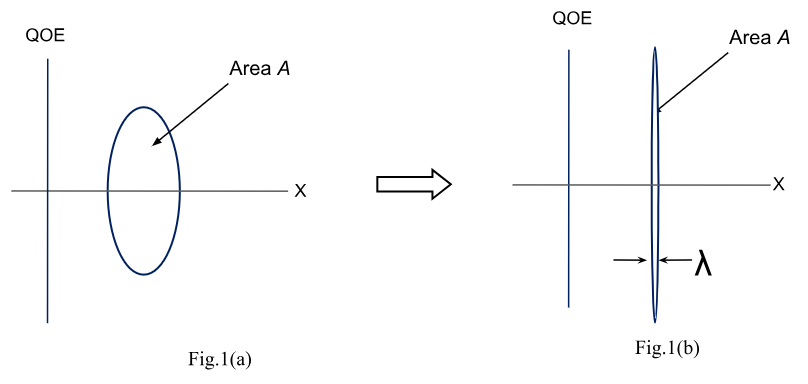
\includegraphics[scale=.5]{images/001.jpg}
\caption{{\fontsize{10}{12}\selectfont {\bf (a):} Phase space area A with oscillatory position x and QOE; {\bf (b)} Phase space area A with position x and more QOE.}}\label{art1-fig1}
\vspace{-.3cm}

\end{figure}

{\fontsize{8}{10}\selectfont\subsection{\textit{Vedantic Tapering Existence and Like Potential Energy (LPE)\\ in QHO – The proposed Vedantic Theory}}}\label{subsec-3.2}

{\fontsize{12}{14}\selectfont If we fix the constant phase space area as the boundary condition, Figure 1 (a) changes into Figure 1 (b), where more energy is infused into the same QHO. The height of the ellipse along the QOE in Figure 1 (a) suggests less energy in the QHO with grosser vibrational displacement along position x. On the other hand, since the phase space area A is kept constant, with more energy in the QHO, the height along the QOE increases, and the vibrational displacement along x decreases, indicating a subtler vibrational state in Figure  1 (b). Following this boundary condition, when we assume infinite energy in the QHO, the vibration becomes zero, showing zero vibrational displacements along the x-axis, and infinite height of the ellipse along the QOE axis. We have discussed before (section 2.1.3) that the vibration or the Nimitta is the cause of both space and time. Hence, at the point when the vibration becomes absolutely zero with the infinite energy in the QHO, there is absolutely no possibility of space-time as well.

Nevertheless, such a state will have infinite energy in the potential form, precisely the same state as the CoP proposed by Vedanta. In this new energy dynamics, the higher energy states correspond to the lower or more potential vibrational states with constant phase space area as the boundary condition. This energy dynamics is termed the Like Potential Energy (hereinafter LPE) dynamics. In other words, it means that under the LPE dynamics, Figure 1 (a) tapers into Figure 1 (b) from grosser to subtler vibrational states with lesser to more energy levels. And finally, this tapering becomes pin-pointed when there is zero vibration with infinite energy. The following figure shows the vibrational tapering with gradually increased energy levels.}

{\fontsize{8}{10}\selectfont\subsubsection{\textit{Consciousness Principle (CoP) from Quantum Harmonic Oscillator (QHO)}}}\label{subsubsec-3.2.1}

{\fontsize{12}{14}\selectfont Figure 2 describes a theoretical relationship between vibration and energy in Like Potential Energy (LPE) dynamics. It suggests less energy with gross vibrations, gradually tapering into infinite energy with zero vibration. The base of the triangle corresponds to the vibration corresponding to all the gross matter in the universe (vibration is the grossest here), and the width x is the oscillation/vibration (displacement) from the equilibrium state of the QHO. The energy of the oscillator QOE is plotted on the y-axis. As the energy increases, following the LPE dynamics, the vibration becomes subtler to finally tapers to zero (where x = 0, and energy reaches infinity at the apex - indicated as CoP).\endnote{In the case of the Big Bang singularity, we may conceive a situation with infinite energy and no vibrational displacement. But we postulate that under the boundary condition of constant phase space area alone, the energy becomes unmanifest as in the Dark Energy, while the Big Bang singularity does not postulate the constant phase space area. In fact, the phase space area in the Big Bang singularity is infinity. This is the difference between the CoP and the Big Bang singularity. The curvature due to LPE is zero, while the curvature due to Big Bang singularity is infinity. Also, the phase space area in LPE is constant, while the phase space area in Big Bang singularity is infinity, the real space area being zero.} Further, the shaded area corresponds to all the gross matter in the universe, including Dark energy and Dark Matter, while the unshaded area corresponds to the world of various subtle matter, like mind, intellect, etc. The transition between gross and subtler matter occurs through the mathematics of LPE dynamics (\underline{Nityayogananda, 2017}) .  This tapering is purely observer specific (\underline{Quantum Theory Demonstrated,1998}) and experienced according to the superimposition of STV on the CoP, the real existence.}

%~ \newpage

\begin{figure}[h]
\centering
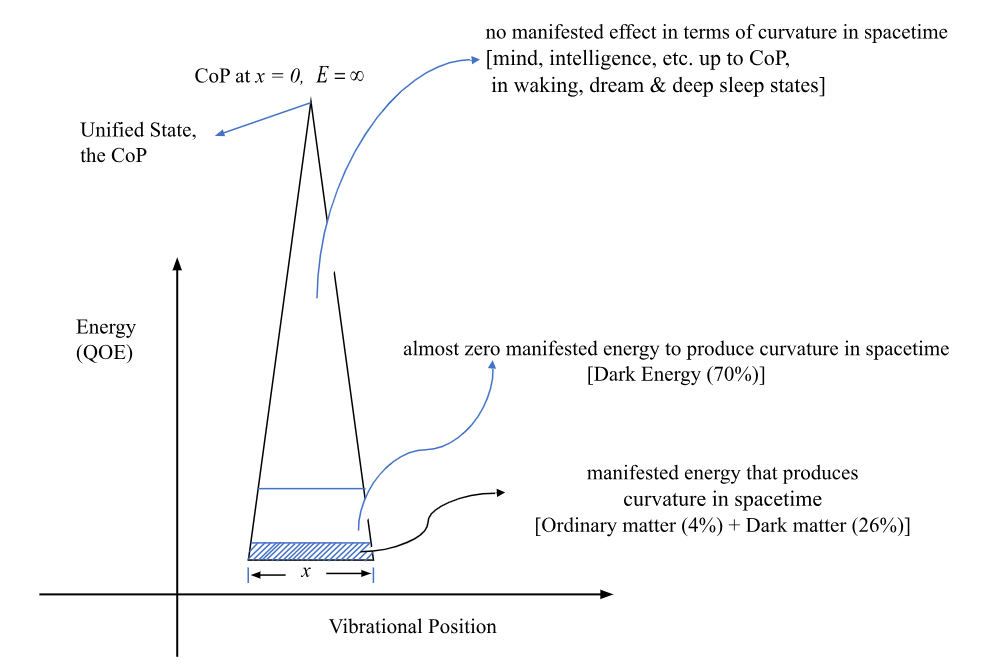
\includegraphics[scale=.43]{images/003.png}
\caption{{\fontsize{10}{12}\selectfont The tapering existence – the subtler the vibration, the more the energy.}}\label{art1-fig2}
\end{figure}

{\fontsize{12}{14}\selectfont First, there is gross matter that is detectable by sense organs such as the eye, touch, etc. And with further tapering, energy becomes subtler and eventually undetectable even by the finest instruments. This continues with an increase in corresponding energy levels until infinity - the CoP state -is finally reached. This undetected portion of energy does not create any curvature in space-time. We have a similar situation in the case of DE, where no curvature is created despite having enormous energy (10$^{113}$ Joules/m$^{3}$). Any form of energy or matter contains the tapering form of existence - tapering from the grosser vibrational existence up to the highest non-vibrational ultimate existence, namely the CoP. Let us consider water as an example. Water can be seen as a combination of hydrogen and oxygen fused under certain conditions. Similarly, it can be considered as the bundle of innumerable QHOs with all quantum fluctuations and energy packets. Again, on further investigation, it can be realized as the CoP (as the yogis perceive).

As per the LPE equation (\underline{Nityayogananda 2017}), the vibration of CoP is infinity in terms of its frequency but zero in terms of displacement. This is what makes CoP have infinite energy but no movement. It is the ever-existent, all-pervasive, beginningless, endless, and immutable CoP in the true sense of the term (since all beginning, end, change etc., are within STV limits only). In other words, it is the CoP that always exists without undergoing any change. But when the ever-existing CoP is superimposed with STV by an observer, the very same CoP appears to that observer to be limited as it manifests into a different energy-matter system that forms the entire cosmos. In actuality, the CoP is the only undivided principle that pervades homogeneously everywhere. There are no two, so to say - two in any sense.\endnote{In a stricter sense, we cannot even say it is ‘One,’ because the idea of ‘One’ arises only when there is the idea of two or many.} And because of its non-physical (thus division-less) nature, we cannot measure the CoP (because to measure anything, we need the STV limit to operate). To measure CoP, it must come under the STV limits (not possible for CoP). We can only propose the CoP theoretically, as has been done here, and realize it subjectively, as innumerable people have verified this realization. This is also subject to verification at all times (as discussed above in section~\ref{subsubsec-2.3.1} under \textit{“VyavahaarikaSatta”}).}

%~ \newpage

{\fontsize{8}{10}\selectfont\subsection{\textit{Energy state from classical (indiscrete)\\ to quantum (discrete) to LPE (indiscrete)}}}\label{subsec-3.3}

%~ \vspace{.1cm}

{\fontsize{12}{14}\selectfont In the classical observable world, the energy, momentum, etc., are observed to be perfectly continuous (indiscrete) and deterministic. When observed in closer detail, {\it i.e.,} on a small scale, the same energy is measured as discrete and probabilistic. The present physics is governed by the quantum states of existence, {\it i.e.,} the small scale, as they are understood to be more fundamental than the classical states. In our study of the LPE dynamics, we postulate that the energy state becomes indiscrete again if still deeper and a higher energy state than that of the quantum state is considered. This indiscrete energy state is the CoP state in the LPE dynamics. All other states in the LPE spectra are discrete states only. This view of CoP to be indiscrete, as obtained by the LPE dynamics, is supported by the Vedantic statement like \foreignlanguage{hindi}{{\fontsize{9}{11}\selectfont “अखण्डएकरसम्”}} \textit{(Akhanda-Ekarasam)} (\underline{Drg-Drsya-Viveka, 1931}) – “the undivided and homogeneous.” The homogeneity in the CoP is due to the indiscrete state of energy. Moreover, as there is a mathematical transition between the classical and quantum states, we propose a mathematical transition between the quantum and the LPE states. This transition is dictated by the boundary condition of the LPE state, namely the constant phase space area. Thus, the subtlest indiscrete state of unmanifested CoP apparently becomes discrete and manifested, and then the same state becomes indiscrete to a certain degree in the gross classical world of measurements.}

{\fontsize{8}{10}\selectfont\subsection{\textit{Space-Time Measurements Redefined with\\ Vibration as the Fifth Dimension}}}\label{subsec-3.4}

\vspace{.1cm}

{\fontsize{12}{14}\selectfont We have seen that vibration plays a pivotal role as the very cause, the \textit{nimitta} of space and time. As per Vedantic conclusion, when the self-willed CoP apparently begins to vibrate, the space and time get their birth.\endnote{Since the whole cosmos is pervaded in and through the CoP, the will of the observer too has a direct connection with the CoP. So, the vibration can be thought of as propagated by the self-willed CoP or as the superimposition by the observer. In any case, both are apparent. The actual CoP is free from all STV triads.} If we can stop all the movements around us through a thought experiment, we can easily understand that the flow of time would also stop at that very instant. And when time stops flowing, space also automatically disappears since space-time forms a single continuum. Thus, it makes sense that there is an intimate connection between vibration, space,  and time to form one single continuum. There will also be the contraction of space due to the vibrational movement. The movement and also the presence of energy body affect the measurement of space and time. In the case of the presence of an energy body, the space and time get curved, and time gets slowed down due to this curvature – more the curvature, slower the time. We propose vibration as an extra dimension, the extension of space-time continuum. This extension of the fifth dimension as the vibration will suitably fit into the Vedantic concept of \textit{Desha-Kala-Nimitta}, as discussed above. Out of these three intimate factors proposed by Vedanta, we have, at present, only \textit{Desha} and \textit{Kala}, {\it i.e.,} space and time to be the single continuum to be called space-time. Here, in apropos Vedantic view, we add the \textit{Nimitta}, {\it i.e.,} the vibration to this space-time continuum and make it a space-time-vibration continuum, or the STV continuum considering the appropriate Action Principle. We have then calculated affine connections in terms of metric tensors in the 5-dimensional pseudo-Riemannian metric space and equated the effect of LPE energy-momentum tensor to zero since the energy-momentum due to LPE does not create any curvature. The detailed mathematical calculations using tensor calculus to extend Einstein’s 4-vector continuum to a 5-vector continuum are shown elsewhere (\underline{Swami Nityayogananda, 2018}). We have also shown there how the LPE with zero curvature can generate a new tensor to explain the anomaly of vacuum catastrophe.}

%~ \newpage

{\fontsize{8}{10}\selectfont\subsection{\textit{The Unified State Theory (UST)}}}

{\fontsize{12}{14}\selectfont As such, vibration does not have as much usage as space-time in our day-to-day measurements. It is because vibration is the background cause \textit{(Nimitta)} to which space-time is the effect. But a deeper theoretical significance can be established by including vibration as a dimension along with space-time. And when we add the LPE tensor and put the vibration to zero to this 5-vector equation, a unified state can be arrived at (\underline{Swami Nityayogananda, 2018}). This unified state is described to be the CoP. Setting vibration as zero, the energy in LPE dynamics reaches infinity. Since this huge energy remains unmanifested under the LPE dynamics, there will not be any space-time curvature due to this huge energy.}

{\fontsize{18}{20}\selectfont\section{Consciousness or Brahman-The Premise of Unification}}\label{sec-4}

\vspace{-.3cm}

{\fontsize{8}{10}\selectfont\subsection{\textit{Consciousness: Vedantic concept}}}\label{subsec-4.1}

{\fontsize{12}{14}\selectfont ‘Consciousness’ or \textit{Chaitanyam} as propounded by the Vedanta is non-physical by nature and exists as the inner essence of the entire universe [as discussed in section 2.3.1 \foreignlanguage{hindi}{{\fontsize{9}{11}\selectfont “यत्साक्षादपरोक्षाद्ब्रह्म, यआत्मासर्वान्तरः”}} \textit{(yat-saakshaat-aparokshaat-brahma, ya-aatmaa-sarvaantarah)}. It is the CoP from which the entire material universe originates (apparently). Vedanta puts it logically that the gross (meaning, the effect) can never produce the subtle (meaning, the cause) because the subtle is more pervasive and lesser limited than the gross, hence cannot be the effect of gross. It is always the subtle that is the cause of the gross; {\it i.e.,} the subtle constituents combine with one another to form the grosser constituents. For example, hydrogen and oxygen combine to form water molecules. Here, in relation to water and hydrogen-oxygen, water is the effect, hence grosser than hydrogen or oxygen. Likewise, the subatomic particles combine with one another to form hydrogen and oxygen atoms. Here, hydrogen and oxygen atoms are grosser than the subatomic particles, etc. Water molecules do not combine to form oxygen and hydrogen atoms.

Alternatively, hydrogen and oxygen atoms do not combine to form subatomic particles. However, water can disintegrate into hydrogen and oxygen, seemingly giving the notion of water producing hydrogen and oxygen. But this, according to Vedanta, is not the production in the true sense. According to Vedanta, an effect (a product) is always the modification and combination of one or many causes. Modifying and combining the subtle or the cause only becomes the gross effect in another form.


Therefore, as we have seen before (under section 2.3, ‘the ultimate substratum’), the conscious cause, {\it i.e.,} Sat projected itself through the STV to become the observer-specific multifarious universe. The regular observation of science also confirms that the subtler energy is more pervasive in power and range than the grosser form of matter. Vedanta’s conclusions are - 1. The CoP exists independent of matter, the STV, 2. The CoP continues to exist even when matter does not exist, 3. The CoP is not the part or product of matter, 4. It is the CoP that pervades matter, not the other way around. According to modern science, as in cognitive neuroscience, the term ‘consciousness’ has a different connotation - which means the individual awareness of a living being (\underline{Michael. S. Gazzaniga, 2018}). On the contrary, the CoP, according to Vedanta, is the ultimate reality, the substratum of the entire cosmos. }

%~ \newpage

{\fontsize{8}{10}\selectfont\subsection{\textit{Unification in Consciousness}}}\label{subsec-4.2}

{\fontsize{12}{14}\selectfont This continuous flux of change occurring in every zepto second is regarded as an illusory existence in Vedanta, suggesting that no physical state, essentially the STV, exists for a single moment (a tiny unit of time tending to zero). This illusory existence is also known as the \textit{VyavahaarikaSatta} (discussed in section 2.3.1). Therefore, this continuous change is happening in every quantum state and every form of gross and subtle matter since matter is only a collection of many quantum states. Although gross matter undergoes constant change, we perceive changelessness in it, albeit temporarily. Vedanta calls this incorrect observation of the world in our daily lives an illusory perception. This continuous change is because of STV.

As described above, the entire phenomenal universe rests on the existence of the STV triad, which itself depends on changeless CoP. Therefore, the ultimate real ‘existence’ is a changeless entity \textit{vis-a-vis} Space, Time, and Vibrations. The CoP alone satisfies these definitions of independent existence, it is the actual bedrock, the substratum of all changeful multiplicities, on which the STV is superimposed, and this STV combination allows all perceivable changes. – \foreignlanguage{hindi}{{\fontsize{9}{11}\selectfont “अद्वयआत्मापरमार्थःसन्प्राणादिविकल्पस्यआस्पदः”}} \textit{(Advaya-aatmaa-paramaarthah-san-praanadivikalpasya- aaspadah)} – “The non-dual Consciousness Principle \textit{(aatma)} is the ultimate reality, the substratum of changing reality as force, etc.” (\underline{Mandukya Upanishad, Agama Prakaranam, introduction 2015}). This changeless CoP is the real ‘Truth’ in an ultimate sense, and all changeful phenomena are unreal. As the Vedanta points out – \foreignlanguage{hindi}{{\fontsize{9}{11}\selectfont “सत्यमितियद्रूपेणयन्निश्चितंतद्रूपंनव्यभिचरति.  यद्रूपेणयन्निश्चितंतद्रूपंव्यभिचरदनृतमित्युच्यते”}} \textit{(“Satyamti-yadroopena-yad-nishchitam-tadroopam-na-vyabhicharati.~Yadroopena-yad\break nishchitam-tadroopam-vyabhicharat-anritam-iti-uchyate”)} – “A thing is said to be \textit{“Sat-\break yam”}, the Truth, when it does not change the nature that is ascertained to be its own. And a thing is said to be unreal when it changes the nature that is ascertained to be its own.” (\underline{Taittiriya Upanishad, Brahmananda Valli 2.1, 2015}). \foreignlanguage{hindi}{{\fontsize{9}{11}\selectfont “चलंशरीरंप्रतिक्षणम्अन्यथाभावात् । अचलम्आत्मतत्त्वम्”}}\textit{(Chalam-shariram-pratikshanam-anyathaabhavaaat. Achalam-aatmatattv-\break am)} – “The inert matter principle \textit{(shariram)} is a changeful entity, for it changes at every moment, while the changeless is the Consciousness Principle” (\underline{Mandukya Upanishad, Va-} \underline{itathyaPrakaranam, Karika 37, 2015}) It is to be noted that some constants in nature, like light speed, gravitational constant etc., are thought to be changeless. However, unlike the CoP, they are not infinity, all-pervasive and non-physical. These constants do depend on STV, while the CoP does not. Hence, these apparently changeless entities in nature are not changeless in the true sense. The perception of the world, including the constants of nature (like light speed, the gravitational constant, etc.), differs from individual to individual due to the varying degrees of STV superimposition in the various body-mind complexes. For example, it is experimentally proven that a common house fly can measure ‘time’ 4 times faster than humans (\underline{Emilie Reas, 2014}). Hence, the measurement of the STV-dependent natural constants also will be different for a housefly from that of humans. As we have discussed above (in section 3.3), there is a possibility that a very tiny creature, almost equal to the size of a quantum particle undergoing statistical fluctuations, may perceive the discrete and fluctuating quantum state to be perfectly indiscrete and deterministic. Also, an enormously big creature, for which our observed classical world may appear to be very small, like a quantum particle, may observe this indiscrete classical world to be discrete and fluctuating. Thus, it can be concluded that the CoP alone satisfies the conditions to be the real and absolute constant. All so-called constants of nature are relative and STV-dependent.

Now, as a thought experiment, if one negates all the changeful entities around (since they do not exist in the real sense of the term, they can be legitimately negated) – first negating the perceived world with all its multiplicities, then negating our own body-mind complex with all its components – we will be finally left with the ‘negator,’ the real observer, the awareness called ‘I.’ Interestingly, this awareness ‘I’ can never be negated, and continues even in other states of our existence, such as dream and deep sleep state, or even in a coma. When a person comes out of deep sleep or from a coma, he/she says, ‘I did not know anything at that state.’ This experience of ‘not-knowing’ ascertains the presence of awareness, {\it i.e.,} ‘I’-ness, during deep sleep or a coma state. Other than the waking state, sense organs (instruments) cannot communicate this subtle awareness to others, mainly due to the unavailability of the instruments of communication, although the CoP remains in those states all the while as awareness or existence. Even in our waking state, all changeful perceptions and intelligent analyses occur over a changeless CoP as the background. It is never ‘Nothing.’ The CoP is like a changeless movie screen onto which all the changeful projections are synchronized. This method of negation to conceive the idea of CoP in the ‘I-ness’ is known as \foreignlanguage{hindi}{{\fontsize{9}{11}\selectfont ‘नेतिनेति’}}  \textit{(Neti Neti)} - “Not just this, not just this” method in Vedanta ({\underline{Brihadaranyaka Upanishad, 2.3.6, 3.8.8, (2015)}). Alternatively, suppose we try to intellectually conceive the constituents (or the cause) of this perceivable universe (or the effect) by a thought experiment. In that case, we will gradually proceed from the grosser to the subtler levels of the phenomenal existence till we come to the STV and finally to the next level, the substratum of everything, namely the CoP. This method to conceive the idea of CoP inferring from the gross material universe is known as \foreignlanguage{hindi}{{\fontsize{9}{11}\selectfont अपवाद}}\textit{(Apavada)} - the de-superimposition in Vedanta (\underline{Vedanta-Sara of Sadananda Yogi, p. 102-104 (2014)}). Vedanta also points out here that mere intellectual understanding of the CoP is not the actual understanding of the Truth. As we have pointed out in section 2.3.1, the words of the Upanishads are taken to be a separate proof called the \textit{ShabdaPramanam} which is different from perception and inference because of their ability to yield a kind of knowledge different from the knowledge yielded by perception and inference. But, as long as we understand those words merely intellectually, those Upanishadic words will fall under perception or inference only. One needs to transcend all the forms of matter, including our intellect (buddhi), to get the knowledge coming out of \textit{ShabdaPramanam}. This knowledge is purely subjective. Any objectification of the CoP with the help of mind, intellect, or any other instrument involves the concept of STV, which is within the realm of matter, not the CoP. The reality is just being and becoming. Swami Vivekananda calls this Vedantic reality the true religion, the unchangeable universal Truth. The true definition of religion in Hindu tradition is the realization of CoP.

Swami Vivekananda’s words in this context are very significant:

%~ \newpage

“The Hindu religion does not consist in struggles and attempts to believe a certain doctrine or dogma, but in realising -- not in believing, but in being and becoming. Thus, the whole object of their system is by constant struggle to become perfect, to become divine, to reach God and see God, and this reaching God, seeing God, becoming perfect even as the Father in Heaven is perfect, constitutes the religion of the Hindus” (\underline{The Complete Works of Swami Vivekananda, Vol. 1 p. 13 (2005)}).\endnote{Our perception of the word ‘religion’ depends on how we define it. According to the definition given by Swami Vivekananda here, also according to the Vedantic conclusion, true religion is a perfect science and must be understood from a scientific viewpoint only. Other commonly used definitions of ‘religion’ do not have much relevance in Vedanta.}

Thus, Vedanta proposes that the world always remains in a unified state (the state of CoP), but due to individual perception, such as STV superimposition on the CoP, the universe is seen/perceived with varieties and changes. Importantly, Vedanta declares that there are not just one but three states of existence that are experienced daily: waking, dreaming, and deep sleep. The dream state experienced by a person appears fully real as experienced in the waking state. Also, in the dream state, the waking state stands negated; in the waking state, the dream state stands negated. Although experienced as three states, the CoP always remains unchanged and unified in all of them in the form of changeless ‘I-ness.’ As discussed before (under section 2.3, ‘the ultimate substratum’), although the body-mind complex undergoes changes from childhood to old age, the sense of ‘I-ness’ remains the same. This changeless ‘I-ness’ is nothing but the CoP, which is all-pervasive, but due to our limited understanding, it is mistakenly thought to be squeezed into a tiny body-mind complex. Based on the unification principle revealed in Vedanta, we conclude that the microcosm (quantum world) and the macrocosm (classical world) are essentially built on the same principles of the CoP and STV triad, as explained above. The only differences between these two states are the gradations of space, time, and vibration superimposed on the CoP and how we observe them.

Vedanta, understood by the LPE dynamics, encompasses every possible existence of the creation into its fold and reaches the grand unification. Thus, Vedanta provides an opportunity to expand the frontier of physics beyond the gross matter experienced by the senses. Perhaps we can explore the possibilities of such unmanifested energy instead of cancelling it as null and void. Such an exercise also considers the mind (mental energy) to be included in physics rather than only in psychological or metaphysical events. What can be a grander unification than this?}

%~ \vspace{-.2cm}

{\fontsize{8}{10}\selectfont\subsection{\textit{Observable dependent External Knowledge – the fallacy\\ of expanding universe}}}\label{subsec-4.3}

{\fontsize{12}{14}\selectfont Before concluding this paper, we will examine a significant data-based event in cosmology and see how the conclusions drawn at different times are widely different due to the difference in collected data. Our knowledge of the universe depends on observational parameters. And the changes in such parameters may lead to different conclusions, significantly impacting our understanding of several natural phenomena. One such crucial natural event is the expansion of the universe. The expansion of the universe is a well-established fact today with no trace of doubt. The speed of a receding galaxy is proportional to its distance from a reference point determined by Hubble law. In other words, the expansion of the universe is accelerated expansion.

As per the astrophysical calculations applying Hubble’s law, the galaxy's speed exceeds the speed of light at the point of ‘horizon’ when observed from the reference frame of our galaxy. Such a phenomenon predicts that we cannot detect/define the occurrences beyond the ‘horizon.’ This also predicts that after about 150 billion years, Andromeda would have collided with ours to form one single galaxy,\endnote{Andromeda galaxy is the single exception coming toward us instead of receding from us. It is because the Milky Way’s gravitational acceleration overpowers the receding acceleration of Andromeda.} and more importantly, no other galaxy would be left within the horizon since all would have departed beyond the horizon. Hence, there will be no reference frame to observe the redshift suggesting the expanding universe. 

Suppose that after 150 billion years from now, Hubble was to observe such an occurrence as the universe's expansion using his latest telescope; he would not be able to identify any redshift because ours would be the only galaxy left within the detectable universe. As an obvious consequence, the cosmological constant relating to the universe’s expansion would lose all its significance, and physicists might offer inconsistent conclusions with reference to today’s understanding of Astrophysics. The concept of the universe's expansion would then be considered a baseless theory. However, the conclusions drawn at that time by observing available data would be perfectly cogent and consistent at that time though altogether different from today’s conclusion. 

Such a proposition demands that scientists be open to accepting/investigating all possible solutions to a given problem. If not, our scientific preparedness may be in question. True science embraces all possible and potential explanations of an observed phenomenon.}


\newpage

{\fontsize{18}{20}\selectfont\section{Promise of the CoP and Future Directions}}\label{sec-5}

\vspace{-.3cm}

{\fontsize{12}{14}\selectfont Knowingly or unknowingly, we are approaching that one state out of which all the phenomenal world has emerged declares the Vedanta. We can understand this by seeing the direction of the journey and progress science is making today. It is our basic instinct to search for unity because unity is what we are, in reality, our essential nature. We get the same question asked in the Upanishad by a student to his teacher to know about a unified state– \foreignlanguage{hindi}{{\fontsize{9}{11}\selectfont “कस्मिन्नुभगवोविज्ञातेसर्वमिदंविज्ञातंभवतीति }}\textit{(kasmin-nu-bhagavo-vijnaate-saravam-idam-vijnaanam-bhavati-it)} – “O Reverend Sir! What is that one thing by knowing which everything in the universe is known?” (\underline{Mundaka Upanishad 1.1.3, 2015}). The answer to this question given by the teacher is – \foreignlanguage{hindi}{{\fontsize{9}{11}\selectfont “यत्तदद्रेश्यमग्राह्यमगोत्रमवर्णमचक्षुःश्रोत्रंतदपाणिपादम्, नित्यंविभुंसर्वगतंसुसूक्ष्मंतदव्ययंयद्भूतयोनिंपरिपश्यन्तिधीराः”}} \textit{(yat-tad-adreshyam-agraahyam-agotram-avarn\break am-achakshuh-shrotram-tad-apaanipaadam, nityam-vibhum-sarvagatam-susukshmam-\break tad-avyayam-yad-bhootayonim-paripashyanti-dheeraah)} – “The wise realize that which cannot be perceived and grasped, which is without source, features, eyes and ears, which has neither hands nor feet, which is eternal, multi-formed (because of assuming diverse forms in all the different creatures), all-pervasive, extremely subtle, and undecaying, and which is the source of all” (\underline{Mundaka Upanishad 1.1.6, 2015}). It is evident from this answer that the ‘one thing’ asked by the student is nothing but the CoP, which is truly the unified state of the entire cosmological phenomena. We have observed here that all the properties of the CoP proposed mathematically in the LPE dynamics correctly match with the Vedantic description of the unified state as mentioned above. These descriptions of unification and reality are found in the Upanishads innumerable times. This search for unification is unquestioned, even as thousands of scientists have dedicated their lives to its pursuit.}

%~ \newpage

%~ \vspace{-.3cm}
{\fontsize{12}{14}\selectfont
\begin{thebibliography}{99}

\bibitem{} Advaita Siddhih by Sri Madhusudana Saraswati, Edited by Pt. Ananta Krishna Sastry, Parimal Publication, Edn. 2014, page 189.

%~ \bibitem{} Advaita Siddhih by Sri Madhusudana Saraswati, 2014.

\bibitem{} Brahmasutra~1.1.2,~commentary of Sri Shankaracharya, Brahmasutra-Sankarabha\break shyam, Edited by Prof.~J.~L.~Shastri, Motilal Banarasidaas, Sanskrit, p.47, 2010.

\bibitem{} Brihadaranyaka Upanishad 3.6.1, 2015.

\bibitem{} Brihadaranyaka Upanishad, commentary, 3.6.1, 2015

\bibitem{} Brihadaranyaka Upanishad 3.7.1, 2015.

\bibitem{} Brihadaranyaka Upanishad 3.6.1, 2015.

\bibitem{} Brihadaranyaka Upanishad 3.7.1, 2015.

\bibitem{} Brihadaranyaka Upanishad 3.4.1, 2015.

\bibitem{} Brihadaranyaka Upanishad, 2.3.6, 3.8.8, (2015).

\bibitem{} Mandukyopanishad Karika, Alatashanti Prakaranam, 2015.

\bibitem{} Brahmasutra commentary, 1.1.2, 2010.

\bibitem{} Brihadaranyaka Upanishad 3.6.1, commentary of Sri Shankaracharya, Ten Principal Upanishads with Sankarabhashyam, Motilal Banarasidaas, Sanskrit, 2015

\bibitem{} Baviskar, A. 2006. Red in Tooth and Claw? Looking for Class in Struggles over Nature In: Ray R and Katzenstein M (Eds.) \textit{Social Movements in India: Poverty, Power and Politics}. (pp. 161-178). Oxford University Press

\bibitem{}Brihadaranyaka Upanishad 3.7.1, Ten Principal Upanishads with Sankarabhashyam, Motilal Banarasidaas, Sanskrit, 2015.

\bibitem{} Brihadaranyaka Upanishad 3.4.1, Ten Principal Upanishads with Sankarabhashyam, Motilal Banarasidaas, Sanskrit, 2015.

\bibitem{} Brihadaranyaka Upanishad 2.3.6, Ten Principal Upanishads with Sankarabhashyam, Motilal Banarasidaas, Sanskrit, 2015.

\bibitem{} Brihadaranyaka Upanishad 3.8.8 Ten Principal Upanishads with Sankarabhashyam, Motilal Banarasidaas, Sanskrit, 2015.

\bibitem{} Chatterjee Satishchandra, “An Introduction to Indian Philosophy”, Rupa \& Co, Dec 2012.

\bibitem{} Chatterjee, 2012.

\bibitem{} Chhandogya Upanishad 6.2.1, Ten Principal Upanishads with Sankarabhashyam, Motilal Banarasidaas, Sanskrit, 2015.

\bibitem{} Chhandogya Upanishad 6.2.1, 2015.

\bibitem{} Drg-Drsya-Viveka: An Inquiry Into The Nature Of The Seer And The Seen, Verse 28, Sankaracharya, Translated By Swami Nikhilananda, Advaita Ashrama, March 1931.

\bibitem{} Drg-Drsya-Viveka, 1931.

\bibitem{} Emilie Reas, “Small Animals Live in a Slow-Motion World” (Scientific American \url{https://www.scientificamerican.com/article/small-animals-live-in-a-slow-motionworld}) (2014). 

\bibitem{} Emilie Reas, 2014.

\bibitem{} Katha Upanishad 6.2, Ten Principal Upanishads with Sankarabhashyam, Motilal Banarasidaas, Sanskrit, 2015.

\bibitem{} Katha Upanishad 6.2, 2015.

\bibitem{} Mandukya Upanishad 8, Ten Principal Upanishads with Sankarabhashyam, Motilal Banarasidaas, Sanskrit, 2015.

\bibitem{} Mandukya Upanishad 6, karika 2, Ten Principal Upanishads with Sankarabhashyam, Motilal Banarasidaas, Sanskrit, 2015.

\bibitem{} Mandukyopanishad Karika, Alatashanti Prakaranam, Karika 47, 48, Ten Principal Upanishads with Sankarabhashyam , Motilal Banarasidaas, Sanskrit, 2015.

\bibitem{} Mandukya Upanishad, Agama Prakaranam, introduction, Shankarabhashyam, Ten Principal Upanishads with Sankarabhashyam, Motilal Banarasidaas, Sanskrit, 2015.

\bibitem{} Mandukya Upanishad, Vaitathya Prakaranam, Karika 37, Shankarabhashyam, Ten Principal Upanishads with Sankarabhashyam, Motilal Banarasidaas, Sanskrit, 2015.

\bibitem{} Mandukya Upanishad 6, karika 2, 2015.

\bibitem{} Michael. S. Gazzaniga, The Consciousness Instinct, Farrar, Straus and Giroux, New York, 2018.

\bibitem{} Michael. S. Gazzaniga, 2018.

%~ \newpage

\bibitem{} Mundaka Upanishad 1.1.3, Ten Principal Upanishads with Sankarabhashyam, Motilal Banarasidaas, Sanskrit, 2015.

\bibitem{} Mundaka Upanishad 1.1.6, Ten Principal Upanishads with Sankarabhashyam, Motilal Banarasidaas, Sanskrit, 2015.

\bibitem{} Mandukya Upanishad 8, 2015.

\bibitem{} Mandukya Upanishad, Agama Prakaranam, introduction 2015.

\bibitem{} Mandukya Upanishad, VaitathyaPrakaranam, Karika 37, 2015.

\bibitem{} Mundaka Upanishad 1.1.3, 2015.

\bibitem{} Mundaka Upanishad 1.1.6, 2015.

\bibitem{} Narlikar V Jayant, “The Scientific Edge – The Indian Scientist from Vedic to modern times”, Penguin Books India, 2003.

\bibitem{} Narlikar, 2003.

\bibitem{} Nityayogananda, S. On quantum harmonic oscillator being subjected to absolute potential state. Pramana phy 88, 4 (2017). \url{https://doi.org/10.1007/s12043-016-1311-x}

\bibitem{} Nityayogananda, 2017.

\bibitem{} Nityayogananda S 2017.

\bibitem{} Nrisimha-uttara-tapaniya Upanishad (\foreignlanguage{hindi}{{\fontsize{9}{11}\selectfont नृसिंह-उत्तर-तापनीयउपनिषद्}}) - 6.2, Anandashrama, Sanskrit, 1929.

\bibitem{} Nrisimha-uttaratapaniya Upanishad, 1929.

\bibitem{} Quantum Theory Demonstrated: Observation Affects Reality, Science Daily, February 1998.

\bibitem{} Quantum Theory Demonstrated,1998.

\bibitem{} Shvetashvetara Upanishad, 6.11, Anandasharama, Motilal Banarasidaas, Sanskrit, 2015.

\bibitem{} Shvetashvetara Upanishad, 6.11, 2015.

\bibitem{} Srimad Bhagavad Gita Ch. 8, verse 19, Swami Vireswarananda, Ramakrishna Math, Mylapore, Chennai, 2nd edition, 2008.

\bibitem{} Srimad Bhagavad Gita Ch.12, verse 3. Swami Vireswarananda, Ramakrishna Math, Mylapore, Chennai, 2nd edition, 2008.

\bibitem{} Srimad Bhagavad Gita Ch. 8, verse 19, 2008.

\bibitem{} Srimad Bhagavad Gita Ch. 12, verse 3, 2008.

\bibitem{} Swami Nityayogananda, “A unified concept of reality: Adding another dimension to Einstein’s field equations”, Global Journal for Research Analysis, Vol. 7, No 10, Oct. 2018.

\bibitem{} Swami Nityayogananda, 2018.

\url{https://www.worldwidejournals.com/global-journal-for-research-analysis-GJRA/fileview/October_2018_1539072247__100.pdf}

\bibitem{} Swami Vivekananda, The Complete Works of Swami Vivekananda, “Cosmology” (Advaita Ashrama Calcutta ISBN 81-85301-76-X) Vol. 2 p, 433 (2005).

\bibitem{} Swami Vivekananda, The Complete Works of Swami Vivekananda (Advaita Ashrama Calcutta ISBN 81-85301-76-X) Vol. 2 p. 427, 440 (2005).

\bibitem{} Swami Vivekananda, The Complete Works of Swami Vivekananda, “Vedic Religious Ideals” (Advaita Ashrama Calcutta ISBN 81-85301-76-X) Vol. 1, p. 351 (2005).

\bibitem{} Swami Vivekananda, The Complete Works of Swami Vivekananda, “Raja-Yoga, Ch3. Prana, (Advaita Ashrama Calcutta ISBN 81-85301-76-X) Vol. 1, p148 (2005).

\bibitem{} Swami Vivekananda, The Complete Works of Swami Vivekananda (Advaita Ashrama Calcutta ISBN 81-85301-76-X) Vol. 2 p 16 (2005).

\bibitem{} Swami Vivekananda, The Complete Works of Swami Vivekananda (Advaita Ashrama Calcutta ISBN 81-85301-76-X) Vol. 1 p13 (2005).

\bibitem{} Swami Vivekananda, The Complete Works of Swami Vivekananda (Advaita Ashrama Calcutta ISBN 81-85301-76-X) Vol. 2 p396 (2005).

\bibitem{} Swami Vivekananda, The Complete Works of Swami Vivekananda (Advaita Ashrama Calcutta ISBN 81-85301-76-X) Vol. 2 p351 (2005).

\bibitem{} The Complete Works of Swami Vivekananda, Vol. 1 p. 351 (2005).

\bibitem{} The Complete Works of Swami Vivekananda, Vol. 1 p. 148 (2005).

\bibitem{} The Complete Works of Swami Vivekananda, Vol. 2 p. 433 (2005).

\bibitem{} The Complete Works of Swami Vivekananda, Vol. 2 p. 427, 440 (2005).

\bibitem{} The Complete Works of Swami Vivekananda, Vol. 2 p. 351 (2005).

\bibitem{} The Complete Works of Swami Vivekananda, Vol. 1, p. 148 (2005).

\bibitem{} The Complete Works of Swami Vivekananda, Vol. 1, p. 148 (2005).

\bibitem{} The Complete Works of Swami Vivekananda, Vol. 2 p. 16 (2005).

\bibitem{} The Complete Works of Swami Vivekananda, Vol. 1 p. 13 (2005).

\bibitem{} The Complete Works of Swami Vivekananda, Vol. 2 p. 396 (2005).

\bibitem{} Taittiriya Upanishad 3.1, Ten Principal Upanishads with Sankarabhashyam, Motilal Banarasidaas, Sanskrit, 2015. 

\bibitem{} Taittiriya Upanishad 2.6, Ten Principal Upanishads with Sankarabhashyam, Motilal Banarasidaas, Sanskrit, 2015.

\bibitem{} Taittiriya Upanishad 3.1, 2015.

\bibitem{} Taittiriya Upanishad 2.6, 2015.

\bibitem{} Taittiriya Upanishad, Brahmananda Valli 2.1, 2015.

\bibitem{} Taittiriya Upanishad, Brahmananda Valli 2.1, Sankarabhashyam, Ten Principal Upanishads with Sankarabhashyam, Motilal Banarasidaas, Sanskrit, 2015.

\bibitem{} Vedanta-Sara of Sadananda Yogi, translated by Swami Nikhilananda, Advaita Ashrama, 7th Edn. p.102-104 (2014).

\bibitem{} Vedanta-Sara of Sadananda Yogi, p. 102-104 (2014).

\end{thebibliography}}}

\theendnotes

\end{document}
